\documentclass[11pt,a4paper]{article}
\usepackage[T1]{fontenc}
\usepackage[utf8]{inputenc}
\usepackage[french]{babel}
\usepackage{geometry}
\usepackage{graphicx}
\usepackage{booktabs}
\usepackage{listings}
\usepackage{hyperref}
\usepackage{float}
\usepackage{longtable}

\geometry{margin=2.2cm}
\hypersetup{colorlinks=true,linkcolor=blue,urlcolor=blue}

\lstset{basicstyle=\ttfamily\small,breaklines=true,frame=single,language=bash}

\title{Rapport technique --- Lab 2\\
\large Campagne paramétrique sur la zone dense Wi-Fi\\
Dépôt \texttt{ns3\_IMT2030\_connectivity}}
\author{Traorehub --- travail de recherche (WIP)}
\date{Novembre 2026}

\begin{document}
\maketitle
\tableofcontents
\newpage

\section{Objectif du laboratoire}

Le Lab 1 a fixé un scénario ns-3 unique et a comparé deux politiques sur quelques points isolés. Le Lab 2 transforme cette comparaison en \textbf{plan d'expérience factoriel}. Les facteurs retenus sont la taille de la grille et l'intervalle entre paquets. La politique reste un facteur à deux niveaux, \texttt{baseline} et \texttt{adaptive}.

L'objectif est de mesurer comment le taux de livraison, l'indice de Jain et le nombre d'événements de gestion varient lorsque la densité et l'intensité temporelle du trafic changent ensemble. Le modèle radio demeure le proxy Wi-Fi 802.11n du Lab 1 (Yans, \texttt{HtMcs7}, SSID \texttt{imt2030-dense-zone}). La durée est fixée à 10~s et chaque terminal prévoit 40 paquets de 512 octets.

\section{Protocole}

Le script \texttt{labs/lab02\_campagne/scripts/lancer\_campagne.py} enchaîne 24 exécutions. Les niveaux sont les suivants.
\begin{itemize}
  \item \texttt{gridSide} dans $\{4, 6, 8, 10\}$, donc 16, 36, 64 et 100 terminaux ;
  \item \texttt{intervalMs} dans $\{40, 80, 160\}$ ;
  \item \texttt{policy} dans $\{\texttt{baseline}, \texttt{adaptive}\}$.
\end{itemize}

L'animation NetAnim est désactivée (\texttt{--enableAnim=0}) afin de limiter le volume des traces. Les lignes sont ajoutées dans \texttt{labs/lab02\_campagne/sorties/resultats.csv}. La colonne \texttt{intervalMs} a été ajoutée au scénario du Lab 1 pour que chaque ligne du CSV soit auto-descriptive. Une graine unique est utilisée, car le scénario ne tire pas encore de répétitions indépendantes.

Le budget de paquets tient dans la fenêtre de simulation pour les trois intervalles. Quarante paquets espacés de 160~ms occupent 6,4~s, ce qui reste inférieur à 10~s. L'offre estimée en octets ne dépend donc pas de l'intervalle. En revanche, le débit offert instantané, qui pilote le rapport $\rho$ du contrôleur, est inversement proportionnel à l'intervalle.

\section{Seuil du contrôleur sur ce plan}

Le contrôleur estime
\[
  \rho = \frac{N_{\mathrm{actifs}}\times 512 \times 8}{\texttt{intervalMs}/1000 \times 8\times 10^{6}}.
\]
Il n'agit que si $\rho > 0{,}82$. Avec la capacité de référence de 8~Mbit/s, ce seuil correspond à environ 6,56~Mbit/s offerts.

Pour 64 terminaux et un intervalle de 40~ms, le débit offert vaut 6,55~Mbit/s, donc $\rho \approx 0{,}819$. Le contrôleur reste inactif, juste sous le seuil. Pour 100 terminaux et 40~ms, le débit offert vaut 10,24~Mbit/s et $\rho \approx 1{,}28$. Le contrôleur s'active. Pour 100 terminaux et 80~ms, $\rho$ retombe à 0,64, et la politique adaptive se confond de nouveau avec la baseline.

\section{Résultats}

\begin{longtable}{@{}rrllrrr@{}}
\caption{Campagne complète, durée 10~s.}\\
\toprule
STA & Intervalle (ms) & Politique & Livraison & Jain & Throttle & Octets reçus \\
\midrule
\endfirsthead
\toprule
STA & Intervalle (ms) & Politique & Livraison & Jain & Throttle & Octets reçus \\
\midrule
\endhead
16 & 40 & baseline & 1,000 & 1,000 & 0 & 327\,680 \\
16 & 40 & adaptive & 1,000 & 1,000 & 0 & 327\,680 \\
16 & 80 & baseline & 1,000 & 1,000 & 0 & 327\,680 \\
16 & 80 & adaptive & 1,000 & 1,000 & 0 & 327\,680 \\
16 & 160 & baseline & 1,000 & 1,000 & 0 & 327\,680 \\
16 & 160 & adaptive & 1,000 & 1,000 & 0 & 327\,680 \\
36 & 40 & baseline & 0,951 & 0,986 & 0 & 701\,440 \\
36 & 40 & adaptive & 0,951 & 0,986 & 0 & 701\,440 \\
36 & 80 & baseline & 0,967 & 0,992 & 0 & 713\,216 \\
36 & 80 & adaptive & 0,967 & 0,992 & 0 & 713\,216 \\
36 & 160 & baseline & 0,973 & 0,993 & 0 & 717\,312 \\
36 & 160 & adaptive & 0,973 & 0,993 & 0 & 717\,312 \\
64 & 40 & baseline & 0,437 & 0,826 & 0 & 572\,928 \\
64 & 40 & adaptive & 0,437 & 0,826 & 0 & 572\,928 \\
64 & 80 & baseline & 0,567 & 0,939 & 0 & 742\,912 \\
64 & 80 & adaptive & 0,567 & 0,939 & 0 & 742\,912 \\
64 & 160 & baseline & 0,625 & 0,977 & 0 & 818\,688 \\
64 & 160 & adaptive & 0,625 & 0,977 & 0 & 818\,688 \\
100 & 40 & baseline & 0,186 & 0,851 & 0 & 381\,440 \\
100 & 40 & adaptive & 0,186 & 0,851 & 50 & 381\,440 \\
100 & 80 & baseline & 0,289 & 0,776 & 0 & 591\,872 \\
100 & 80 & adaptive & 0,289 & 0,776 & 0 & 591\,872 \\
100 & 160 & baseline & 0,354 & 0,819 & 0 & 724\,480 \\
100 & 160 & adaptive & 0,354 & 0,819 & 0 & 724\,480 \\
\bottomrule
\end{longtable}

\begin{figure}[H]
  \centering
  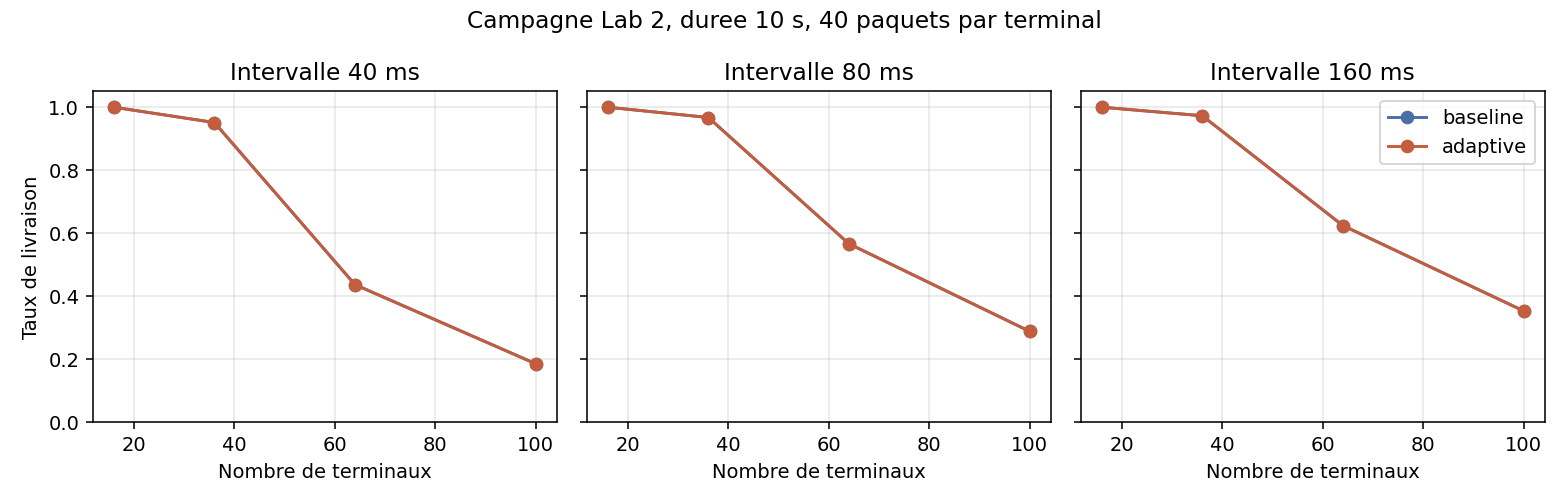
\includegraphics[width=\linewidth]{../../labs/lab02_campagne/sorties/livraison_campagne.png}
  \caption{Taux de livraison en fonction du nombre de terminaux, pour chaque intervalle. Les courbes baseline et adaptive coïncident sur les 24 runs, car le contrôleur ne modifie pas les octets reçus.}
\end{figure}

\begin{figure}[H]
  \centering
  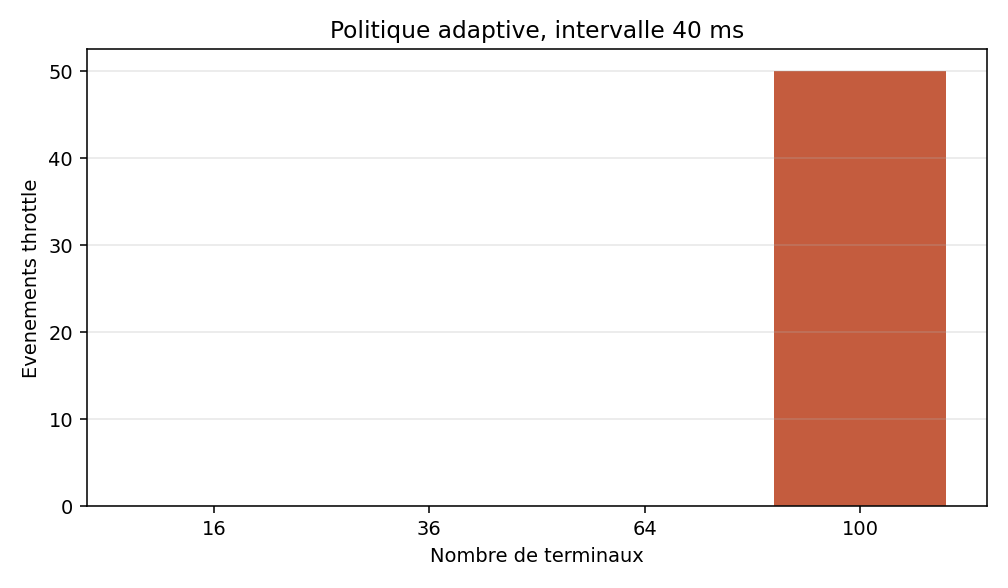
\includegraphics[width=0.72\linewidth]{../../labs/lab02_campagne/sorties/throttle_40ms.png}
  \caption{Événements de gestion de la politique adaptive lorsque l'intervalle vaut 40~ms. Seule la grille de 100 terminaux déclenche le contrôleur.}
\end{figure}

\section{Interprétation}

Sur 16 terminaux, la livraison est totale et l'indice de Jain vaut 1 pour les trois intervalles. Le canal absorbe le budget de 40 paquets par station. La politique adaptive n'a aucune raison de s'activer, et les deux colonnes du tableau coïncident.

Sur 36 terminaux, une légère perte apparaît. La livraison passe de 0,951 à 40~ms jusqu'à 0,973 à 160~ms. Étaler le même nombre de paquets dans le temps réduit la contention. L'effet reste modéré, et le contrôleur demeure inactif.

Sur 64 terminaux, la livraison devient sensible à l'intervalle. Elle vaut 0,437 à 40~ms, 0,567 à 80~ms et 0,625 à 160~ms. L'indice de Jain suit la même progression, de 0,826 à 0,977. Le point à 40~ms est particulièrement instructif pour le contrôleur. Le débit offert se situe juste sous le seuil 0,82, donc la politique adaptive ne produit aucun événement, alors que le canal Wi-Fi est déjà fortement saturé. Le seuil heuristique et la saturation réelle du médium ne coïncident pas.

Sur 100 terminaux, la livraison tombe à 0,186 lorsque les paquets sont rapprochés de 40~ms. Elle remonte à 0,289 à 80~ms et à 0,354 à 160~ms, tout en restant basse. Le seul cas où \texttt{throttleEvents} vaut 50 est la combinaison 100 terminaux et 40~ms en mode adaptive. Les octets reçus et l'indice de Jain restent identiques à ceux de la baseline. Le contrôleur enregistre donc des actions sans modifier, sur cette version, la métrique de service.

L'indice de Jain à 100 terminaux et 80~ms vaut 0,776, ce qui est inférieur à la valeur 0,851 observée à 40~ms. La livraison augmente lorsque l'intervalle passe de 40 à 80~ms, tandis que l'équité mesurée par FlowMonitor se dégrade légèrement. Les deux indicateurs ne racontent pas la même histoire, et une conclusion limitée au seul taux de livraison serait incomplète.

\section{Conséquence pour la suite}

Le plan factoriel montre que la densité et l'espacement temporel des paquets dominent les métriques du Lab 1. Le contrôleur de la version 0 ne s'écarte de la baseline que dans une cellule du plan, et il n'y modifie pas la livraison. Le Lab 3 devra donc déplacer le seuil, ou compter l'offre réellement encore en vol, de façon à agir avant que le canal soit déjà saturé, puis vérifier le gain sur \texttt{deliveryRatio} à l'aide du même plan.

La campagne repose sur une seule graine. Une répétition avec plusieurs \texttt{RngRun} reste nécessaire avant toute affirmation statistique sur de petits écarts, par exemple l'écart de Jain entre 40 et 80~ms à 100 terminaux.

\section{Reproduction}

\begin{lstlisting}
cd /mnt/c/Users/MOH/Documents/Projet_Perso/ns-allinone-3.43
python3 projet-visuel-imt2030/labs/lab02_campagne/scripts/lancer_campagne.py
python3 projet-visuel-imt2030/labs/lab02_campagne/scripts/analyser_campagne.py
cd projet-visuel-imt2030/docs/latex
pdflatex rapport_lab02.tex
pdflatex rapport_lab02.tex
\end{lstlisting}

Le premier script suppose que le binaire scratch a été compilé dans \texttt{ns-3.43}. Il relance la compilation si le source a changé.

\end{document}
